\documentclass[border=4pt]{standalone}
\usepackage{tikz}
\usepackage{lmodern}
\renewcommand{\familydefault}{\sfdefault}
\definecolor{amd}{HTML}{8A8F98}\definecolor{intel}{HTML}{2F6DB5}\definecolor{load}{HTML}{C46A1B}
\begin{document}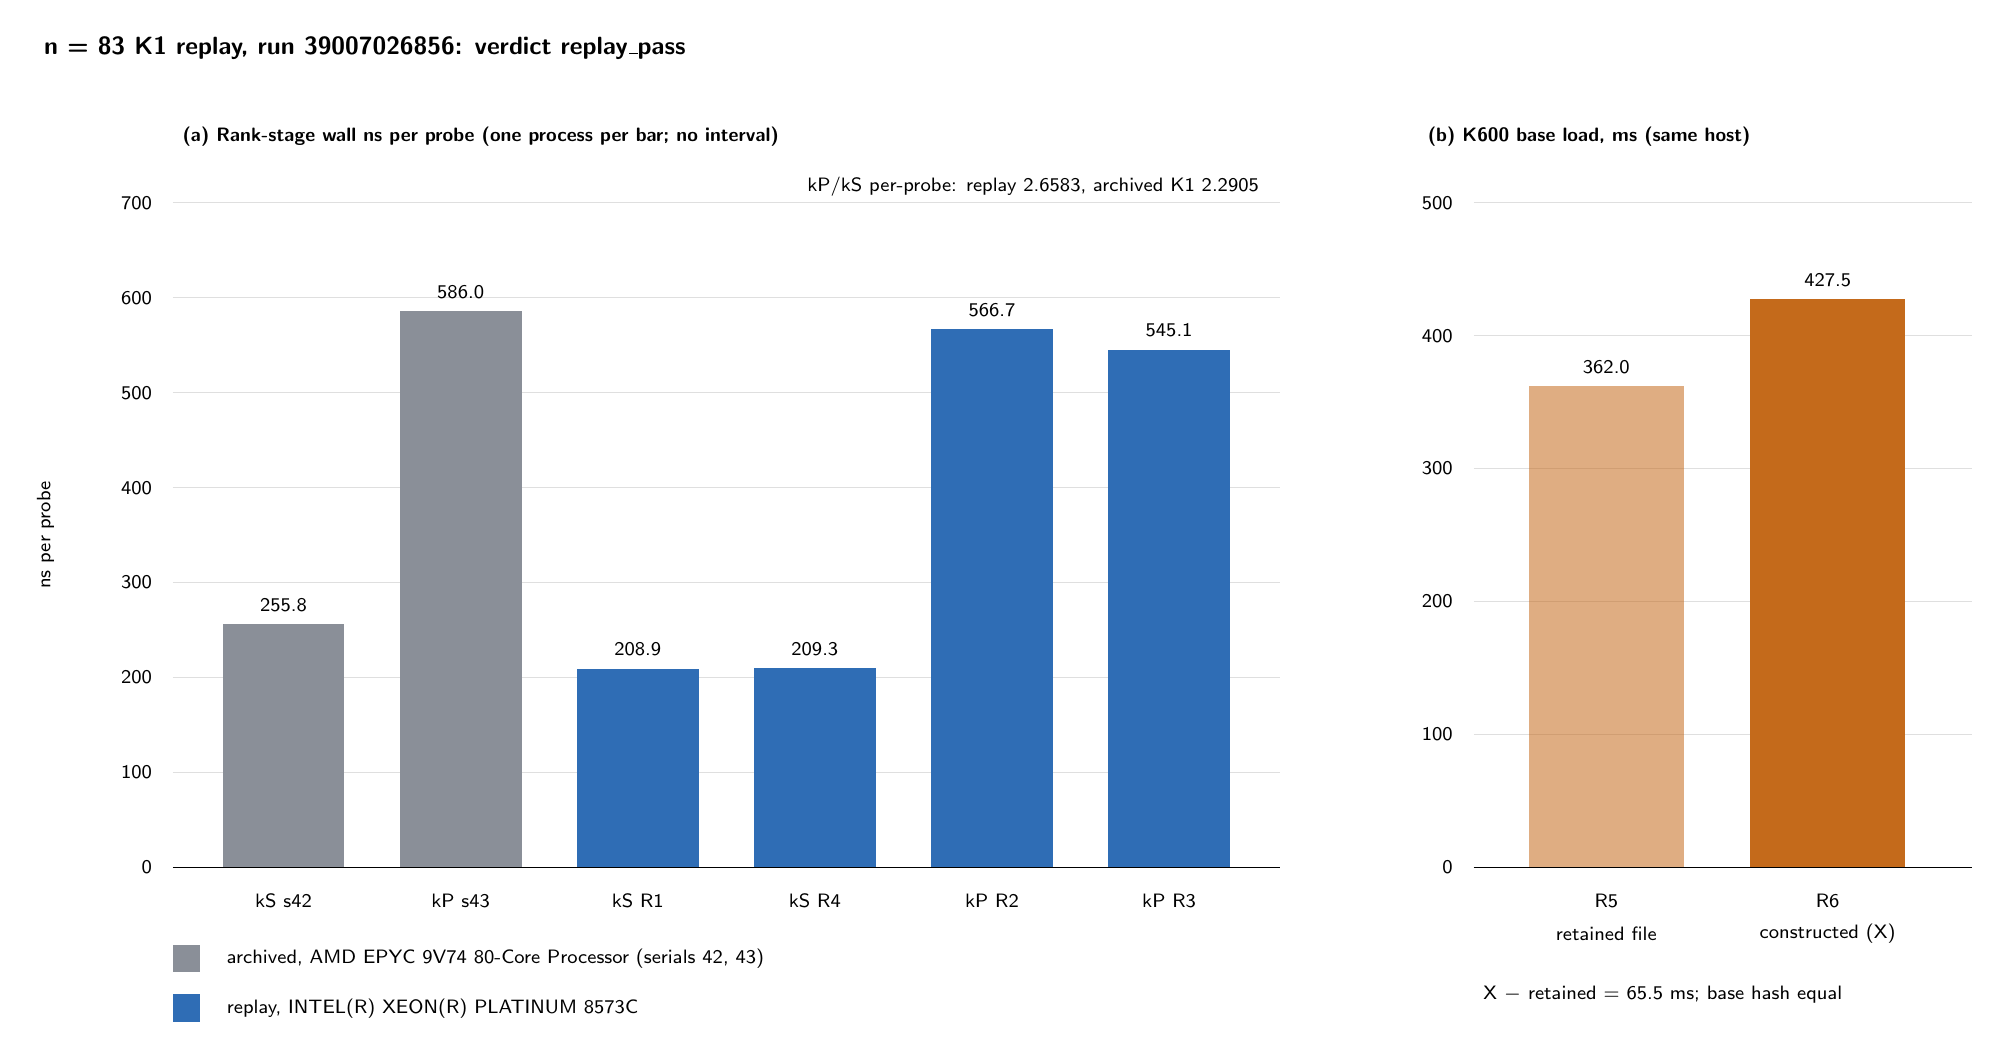
\begin{tikzpicture}[x=1pt,y=-1pt,font=\scriptsize]
\node[anchor=west,font=\small\bfseries] at (20,24) {n = 83 K1 replay, run 39007026856: verdict replay\_pass};
\node[anchor=west,font=\scriptsize\bfseries] at (70,56) {(a) Rank-stage wall ns per probe (one process per bar; no interval)};
\draw[gray!25] (70,320.0) -- (470,320.0); \node[anchor=east] at (66,320.0) {0};
\draw[gray!25] (70,285.7) -- (470,285.7); \node[anchor=east] at (66,285.7) {100};
\draw[gray!25] (70,251.4) -- (470,251.4); \node[anchor=east] at (66,251.4) {200};
\draw[gray!25] (70,217.1) -- (470,217.1); \node[anchor=east] at (66,217.1) {300};
\draw[gray!25] (70,182.9) -- (470,182.9); \node[anchor=east] at (66,182.9) {400};
\draw[gray!25] (70,148.6) -- (470,148.6); \node[anchor=east] at (66,148.6) {500};
\draw[gray!25] (70,114.3) -- (470,114.3); \node[anchor=east] at (66,114.3) {600};
\draw[gray!25] (70,80.0) -- (470,80.0); \node[anchor=east] at (66,80.0) {700};
\node[rotate=90] at (24,200.0) {ns per probe};
\fill[amd] (88,320) rectangle (132,232.3); \node at (110.0,225.3) {255.8}; \node at (110.0,332) {kS s42};
\fill[amd] (152,320) rectangle (196,119.1); \node at (174.0,112.1) {586.0}; \node at (174.0,332) {kP s43};
\fill[intel] (216,320) rectangle (260,248.4); \node at (238.0,241.4) {208.9}; \node at (238.0,332) {kS R1};
\fill[intel] (280,320) rectangle (324,248.2); \node at (302.0,241.2) {209.3}; \node at (302.0,332) {kS R4};
\fill[intel] (344,320) rectangle (388,125.7); \node at (366.0,118.7) {566.7}; \node at (366.0,332) {kP R2};
\fill[intel] (408,320) rectangle (452,133.1); \node at (430.0,126.1) {545.1}; \node at (430.0,332) {kP R3};
\draw (70,320) -- (470,320);
\fill[amd] (70,348) rectangle +(10,10); \node[anchor=west] at (86,353) {archived, AMD EPYC 9V74 80-Core Processor (serials 42, 43)};
\fill[intel] (70,366) rectangle +(10,10); \node[anchor=west] at (86,371) {replay, INTEL(R) XEON(R) PLATINUM 8573C};
\node[anchor=east] at (466,74) {kP/kS per-probe: replay 2.6583, archived K1 2.2905};
\node[anchor=west,font=\scriptsize\bfseries] at (520,56) {(b) K600 base load, ms (same host)};
\draw[gray!25] (540,320.0) -- (720,320.0); \node[anchor=east] at (536,320.0) {0};
\draw[gray!25] (540,272.0) -- (720,272.0); \node[anchor=east] at (536,272.0) {100};
\draw[gray!25] (540,224.0) -- (720,224.0); \node[anchor=east] at (536,224.0) {200};
\draw[gray!25] (540,176.0) -- (720,176.0); \node[anchor=east] at (536,176.0) {300};
\draw[gray!25] (540,128.0) -- (720,128.0); \node[anchor=east] at (536,128.0) {400};
\draw[gray!25] (540,80.0) -- (720,80.0); \node[anchor=east] at (536,80.0) {500};
\fill[load,opacity=0.55] (560,320) rectangle (616,146.2); \node at (588,139.2) {362.0}; \node at (588,332) {R5}; \node at (588,344) {retained file};
\fill[load,opacity=1] (640,320) rectangle (696,114.8); \node at (668,107.8) {427.5}; \node at (668,332) {R6}; \node at (668,344) {constructed (X)};
\draw (540,320) -- (720,320);
\node[anchor=west] at (540,366) {X $-$ retained = 65.5 ms; base hash equal};
\end{tikzpicture}\end{document}
